\documentclass[letterpaper, 11pt]{article}
\usepackage[margin=1in]{geometry}

% Set the typeface to Times Roman
\usepackage{times}

%\usepackage{hyperref}
\usepackage{amsfonts}%
\usepackage{amssymb}%
\usepackage{amsthm}% allows theoremstyles (see below) and provides a proof environment
\usepackage{bm}
\usepackage{relsize}
\usepackage{graphicx}
\usepackage{caption}
\usepackage{epstopdf}
\usepackage{amsmath}
\usepackage{tikz}
\usetikzlibrary{trees,arrows}
\usetikzlibrary{decorations}
\usetikzlibrary[decorations]
\usepgflibrary{decorations.pathmorphing}
\usepgflibrary[decorations.pathmorphing]
\usetikzlibrary{decorations.pathmorphing}
\usetikzlibrary[decorations.pathmorphing]
\usepackage{booktabs}
\usepackage[authoryear]{natbib}
\usepackage{subcaption}
\usepackage{algorithm}
\usepackage[noend]{algpseudocode}
\usepackage{pseudocode}
%\usepackage{float}
\usepackage{verbatim} %% for commenting blocks
\usepackage[authoryear]{natbib}
\usepackage{url}

\bibpunct{(}{)}{,}{}{}{;} %% added this to make \citep{x} use parentheses

\newcommand{\problemAnswer}[1]{%#1% Defines the problem answer command with the content as the only argument
\noindent\framebox[0.95\columnwidth][c]{\begin{minipage}{0.92\columnwidth}\color{blue}{#1}\end{minipage}} % Makes the box around the problem answer and puts the content inside
}

%% independence symbol and expectation operator %%
\newcommand\independent{\protect\mathpalette{\protect\independenT}{\perp}}
\def\independenT#1#2{\mathrel{\rlap{$#1#2$}\mkern2mu{#1#2}}}

\DeclareMathOperator{\circlearrow}{\hbox{$\circ$}\kern-1.5pt\hbox{$\rightarrow$}}
\DeclareMathOperator{\circlecircle}{\hbox{$\circ$}\kern-1.2pt\hbox{$--$}\kern-1.5pt\hbox{$\circ$}}

\DeclareMathOperator{\an}{an}
\DeclareMathOperator{\pa}{pa}
\DeclareMathOperator{\ch}{ch}
\DeclareMathOperator{\pre}{pre}
\DeclareMathOperator{\de}{de}
\DeclareMathOperator{\nd}{nd}
\DeclareMathOperator{\nb}{nb}
\DeclareMathOperator{\pan}{pan}
\DeclareMathOperator{\sib}{sib}
\DeclareMathOperator{\dis}{dis}
\DeclareMathOperator{\mb}{mb}
\DeclareMathOperator{\doo}{do}
\DeclareMathOperator{\odds}{\text{OR}}
\DeclareMathOperator*{\argmax}{arg\,max}
\DeclareMathOperator*{\argmin}{arg\,min}
\definecolor{lemon}{RGB}{ 242, 200,  24}
\def\ci{\perp\!\!\!\perp}
\newcommand{\E}{\mathbb{E}}
\newcommand{\G}{\mathcal{G}}

\newcommand\indep{\protect\mathpalette{\protect\independenT}{\perp}}
\def\independenT#1#2{\mathrel{\rlap{$#1#2$}\mkern2mu{#1#2}}}

\newtheorem{Lma}{Lemma}
\newtheorem{Thm}{Theorem}

\DeclareMathOperator{\diedgeright}{\textcolor{blue}{\boldsymbol{\rightarrow}}}
\DeclareMathOperator{\diedgeleft}{\textcolor{blue}{\boldsymbol{\leftarrow}}}
\DeclareMathOperator{\biedge}{\textcolor{red}{\boldsymbol{\leftrightarrow}}}
\DeclareMathOperator{\udedge}{\textcolor{brown}{\boldsymbol{\textendash}}}
%%%%%%%%%%%%%%%%%%%%%%%%%%%%

\title{CS 476/676 (Spring 2021): Homework 3}

\author{}

\date{Due: Mar 3, 2021 at 11:59pm EST}

\begin{document}

\maketitle

\setlength{\parindent}{0em}
\setlength{\parskip}{0.8em}

\large\textbf{Name:} \underline{\hspace{30pt} \color{blue} Joshua Popp \hspace{30pt}}
\vspace{1em}

	\textbf{Instructions}: This homework requires answering some open-ended questions, short proofs, and
	programming. This is an individual assignment, not group work. Though you may
	discuss the problems with your classmates, you must solve the problems and
	write the solutions independently. As stated in the syllabus, copying code
	from a classmate or the internet (even with minor changes) constitutes
	plagiarism. You are required to submit your answers in pdf form (use \LaTeX)
	in a file called \texttt{<your-JHED>-hw3.pdf} to Gradescope under ``HW3''. Code should be submitted also to Gradescope under ``HW3 Programming''. Note that the autograder setup is intended only to register submission of the code, and will not provide any feedback. Code grading will be performed manually.
	Late submissions will be penalized, except in extenuating circumstances such
	as medical or family emergency. Submissions submitted 0-24 hours late will be
	penalized 10\%, 24-48 hours late by 20\%, 48-72 hours late by 30\%, and later
    than 72 hours by 100\%. Late days may be used (if available) to avoid these penalties.

    The total assignment is worth 80 points + up to 6 points of extra credit.

    \textbf{Important note:} For drawing graphs on this assignment, we  encourage you to use the \LaTeX\  template provided to draw graphs using the \texttt{tikz} package. However, hand drawing graphs/using other software and then including the images into the pdf using \texttt{includegraphics} is also acceptable as long as it is neat.

    \textbf{Important note:} For the non-programming portions of the assignment that require drawing graphs, we  encourage you to use the \LaTeX\  template provided to draw graphs using the \texttt{tikz} package. However, hand drawing graphs/using other software and then including the images into the pdf using \texttt{includegraphics} is also acceptable as long as it is neat. For the programming portion, you \textbf{must} use a software package to produce a graphical visualization of the output of your code.

    As an example of such external software that may produce acceptable results, you may consider using the \texttt{Ananke} Python package to draw undirected graphs, chain graphs and directed acyclic graphs. We have provided an example of its usage in the \texttt{hw3.py} code skeleton. \\[0.5 em]
    \url{https://ananke.readthedocs.io/en/latest/index.html} for installation and overview. \\
    \url{https://ananke.readthedocs.io/en/latest/notebooks/causal_graphs.html} \\for how to draw various classes of graphs.

\vspace{2em}

{\large\textbf{Problem 1}} (6 points)

Consider an undirected graph $\G$ on defined over $d$ variables $V_1, \dots, V_d$. The clique factorization of UGs states that each clique potential must be \textbf{non-negative}. We claim that the odds ratio factorization of UGs is equivalent to the clique factorization. This must mean that the 1-way, 2-way, 3-way, $\dots$, $d$-way terms that appear in the odds ratio factorization satisfy the non-negativity constraint. Prove that this is true. A simple inductive argument for higher order terms (greater than 2-way interactions) will suffice.

\problemAnswer{
Taking a reference value of 0 for each $V_1, V_2, ..., V_d \in V$ as in class, our odds ratio factorization of $p(V)$ is as follows
\begin{align*}
p(V) &= \frac1Z \times \prod_{V_i \in V} p \big( V_i \mid \nb_\G(V_i)=0) \\
& \times \prod_{ \{ V_i, V_j \} \in V} \odds \big( V_i, V_j \mid \nb_\G(V_i, V_j)=0 \big) \\
& \times \text{higher order terms}
\end{align*}
Our normalization constant $Z$ is non-negative by design, this is simply a positive factor taken to ensure our distribution is a valid probability distribution. Each first-order term is in itself a probability distribution, so
$p \big( V_i \mid \nb_\G(V_i)=0) \in [0, 1] \implies p \big( V_i \mid \nb_\G(V_i)=0) \geq 0 \ \forall V_i \in V$. Second order terms consist of the odds ratio,
$$ \odds \big( V_i, V_j \mid \nb_\G(V_i, V_j)=0 \big) $$
which we can also break down into the product of first-order probabilities using the definition of the odds ratio
\begin{align*}
 \odds \big( V_i, V_j \mid \nb_\G(V_i, V_j)=0 \big) &= \frac{p(V_i=x \mid V_j = y, \nb_\G(V_i, V_j)=0)}{p(V_i=0 \mid V_j = y, \nb_\G(V_i, V_j)=0)}\\
 &\times \frac{p(V_i=0 \mid V_j = 0, \nb_\G(V_i, V_j)=0)}{p(V_i=x \mid V_j = 0, \nb_\G(V_i, V_j)=0)}
 \end{align*}
Note that in this example, we take reference values of 0. We cannot obtain negative numbers through the multiplication/ division of non-negative numbers, and this demonstrates that any odds ratio can be expressed as the product/ division of first-order probabilities, which are non-negative. Any higher order terms can be expressed by multiplying/ dividing pairwise odds ratios as demonstrated in class, so by induction these too can be decomposed into the product/ division of non-negative numbers, and consequently cannot break the non-negativity constraint.
}

\vspace{1em}

{\large\textbf{Problem 2}} (13 points)

\begin{figure}[h]
	\begin{center}
		\scalebox{0.8}{
			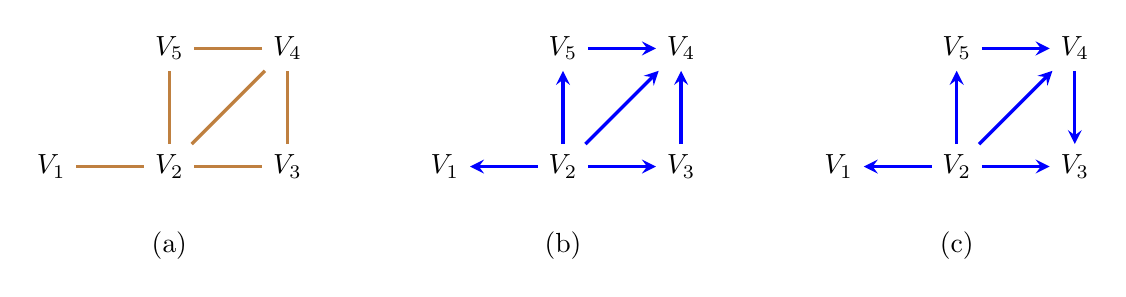
\begin{tikzpicture}[>=stealth, node distance=1.5cm]
			\tikzstyle{format} = [draw, thick, circle, minimum size=1.0mm, inner sep=0pt]
			\tikzstyle{square} = [draw, thick, minimum size=1.0mm, inner sep=3pt]
			\begin{scope}
			\path[->, very thick]
			node[] (v1) {$V_1$}
			node[right of=v1] (v2) {$V_2$}
			node[right of=v2] (v3) {$V_3$}
			node[above of=v3] (v4) {$V_4$}
			node[left of=v4] (v5) {$V_5$}
			node[below of=v2, yshift=0.5cm] (label) {(a)}

			(v1) edge[brown, -] (v2)
			(v2) edge[brown, -] (v3)
			(v3) edge[brown, -] (v4)
			(v4) edge[brown, -] (v5)
			(v2) edge[brown, -] (v4)
			(v2) edge[brown, -] (v5)
			;
			\end{scope}

			\begin{scope}[xshift=5cm]
			\path[->, very thick]
			node[] (v1) {$V_1$}
			node[right of=v1] (v2) {$V_2$}
			node[right of=v2] (v3) {$V_3$}
			node[above of=v3] (v4) {$V_4$}
			node[left of=v4] (v5) {$V_5$}
			node[below of=v2, yshift=0.5cm] (label) {(b)}

			(v2) edge[blue] (v1)
			(v5) edge[blue] (v4)
			(v2) edge[blue] (v4)
			(v3) edge[blue] (v4)
			(v2) edge[blue] (v3)
			(v2) edge[blue] (v5)
			;
			\end{scope}

			\begin{scope}[xshift=10cm]
			\path[->, very thick]
			node[] (v1) {$V_1$}
			node[right of=v1] (v2) {$V_2$}
			node[right of=v2] (v3) {$V_3$}
			node[above of=v3] (v4) {$V_4$}
			node[left of=v4] (v5) {$V_5$}
			node[below of=v2, yshift=0.5cm] (label) {(c)}

			% simplicial ordering v1, v3, v4, v5, v2, v1
			(v2) edge[blue] (v1)
			(v2) edge[blue] (v3)
			(v4) edge[blue] (v3)
			(v5) edge[blue] (v4)
			(v2) edge[blue] (v4)
			(v2) edge[blue] (v5)
			;
			\end{scope}

			\end{tikzpicture}
		}
	\end{center}
	\caption{}
	\label{fig:prob1}
\end{figure}

Refer to Figure~\ref{fig:prob1} for this problem.

1) Briefly describe the graphical property that the UG in Figure~\ref{fig:prob1}(a) satisfies, which allows it to be represented by a Markov equivalent DAG. (3 points)

\problemAnswer{
This is a chordal graph, meaning that any cycles of length 4 or greater (in this case, just $V_2-V_3-V_4-V_5$) contains a chord
}

2) One of the DAGs in Figure~\ref{fig:prob1} (b) or (c) is \textbf{not} Markov equivalent to the UG in (a) -- prove which one by demonstrating a separation that holds in (a) via u-separation but not in (c) via d-separation. (5 points)

\problemAnswer{
(b) is not Markov equivalent to the UG as $V_3 \ci V_5 \mid V_4$ in (a) but not in (b) due to a collider
}

3) On careful examination, you will notice that the DAG chosen as the answer to part 2) has no Markov equivalent UG representation. What is the graphical property of this DAG that prevents this? Confirm that the other DAG does not have this issue. (5 points)

\problemAnswer{
The DAG in (b) has an unshielded collider $V_3 \diedgeright V_4 \diedgeleft V_5$ (meaning there exists no direct edge $V_3 \diedgeright V_5$ nor $V_3 \diedgeleft V_5$).(c) does not have this issue. There are colliders at $V_3$ ($V_2 \diedgeright V_3 \diedgeleft V_4$) and $V_4$ ($V_2 \diedgeright V_4 \diedgeleft V_5$) but both of these have an edge between the co-parents ($V_2 \diedgeright V_4$ and $V_2 \diedgeright V_5$) so they are shielded.
}

\vspace{2em}

{\large\textbf{Problem 3}} (15 points)

\begin{figure}[t]
	\begin{center}
		\scalebox{0.9}{
			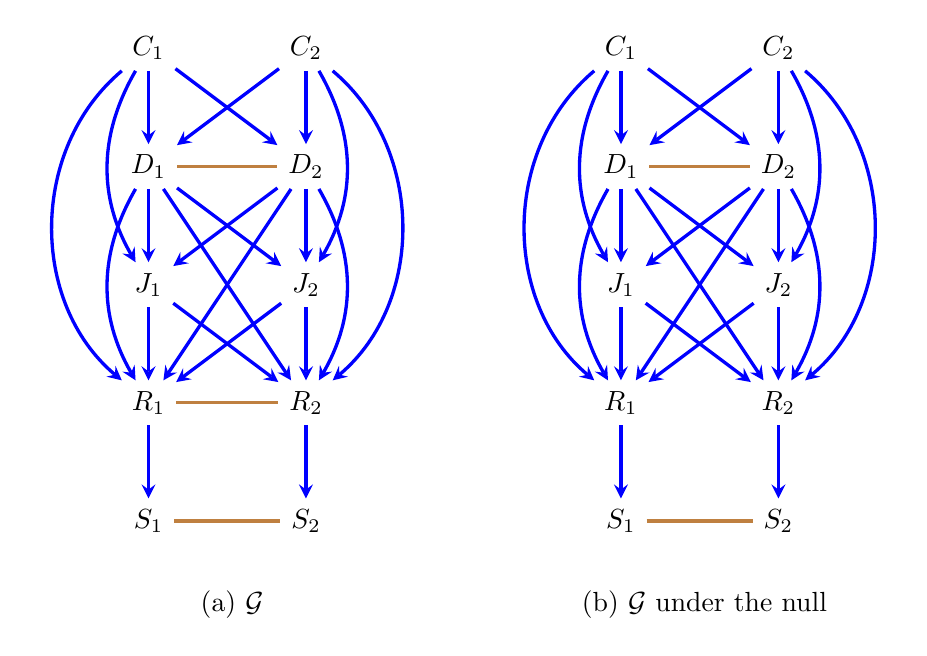
\begin{tikzpicture}[>=stealth, node distance=1.5cm]
			\tikzstyle{format} = [very thick, minimum size=5.0mm, inner sep=0pt]
			\tikzstyle{square} = [draw, very thick, rectangle, minimum size=5.0mm, inner sep=0pt]

			\begin{scope}
			\path[->, very thick]
			node[] (c1) {$C_1$}
			node[below of=c1] (d1) {$D_1$}
			node[below of=d1] (j1) {$J_1$}
			node[below of=j1] (r1) {$R_1$}
			node[below of=r1] (s1) {$S_1$}

			node[right of=c1, xshift=0.5cm] (c2) {$C_2$}
			node[below of=c2] (d2) {$D_2$}
			node[below of=d2] (j2) {$J_2$}
			node[below of=j2] (r2) {$R_2$}
			node[below of=r2] (s2) {$S_2$}
			node[below right of=s1] (label) {(a) $\G$}

			(c1) edge[blue] (d1)
			(d1) edge[blue] (j1)
			(j1) edge[blue] (r1)
			(r1) edge[blue] (s1)
			(c1) edge[blue, bend right] (j1)
			(c1) edge[blue, bend right=50] (r1)
			(d1) edge[blue, bend right] (r1)

			(c2) edge[blue] (d2)
			(d2) edge[blue] (j2)
			(j2) edge[blue] (r2)
			(r2) edge[blue] (s2)
			(c2) edge[blue, bend left] (j2)
			(c2) edge[blue, bend left=50] (r2)
			(d2) edge[blue, bend left] (r2)
			(d1) edge[-, brown] (d2)
			(c1) edge[blue] (d2)
			(c2) edge[blue] (d1)

			(r1) edge[-, brown] (r2)
			(s1) edge[-, brown] (s2)
			(d1) edge[blue] (j2)
			(d2) edge[blue] (j1)
			(d1) edge[blue] (r2)
			(d2) edge[blue] (r1)
			(j1) edge[blue] (r2)
			(j2) edge[blue] (r1)
			;
			\end{scope}

			\begin{scope}[xshift=6cm]
			\path[->, very thick]
			node[] (c1) {$C_1$}
			node[below of=c1] (d1) {$D_1$}
			node[below of=d1] (j1) {$J_1$}
			node[below of=j1] (r1) {$R_1$}
			node[below of=r1] (s1) {$S_1$}

			node[right of=c1, xshift=0.5cm] (c2) {$C_2$}
			node[below of=c2] (d2) {$D_2$}
			node[below of=d2] (j2) {$J_2$}
			node[below of=j2] (r2) {$R_2$}
			node[below of=r2] (s2) {$S_2$}
			node[below right of=s1] (label) {(b) $\G$ under the null}

			(c1) edge[blue] (d1)
			(d1) edge[blue] (j1)
			(j1) edge[blue] (r1)
			(r1) edge[blue] (s1)
			(c1) edge[blue, bend right] (j1)
			(c1) edge[blue, bend right=50] (r1)
			(d1) edge[blue, bend right] (r1)

			(c2) edge[blue] (d2)
			(d2) edge[blue] (j2)
			(j2) edge[blue] (r2)
			(r2) edge[blue] (s2)
			(c2) edge[blue, bend left] (j2)
			(c2) edge[blue, bend left=50] (r2)
			(d2) edge[blue, bend left] (r2)
			(d1) edge[-, brown] (d2)
			(c1) edge[blue] (d2)
			(c2) edge[blue] (d1)

			(s1) edge[-, brown] (s2)
			(d1) edge[blue] (j2)
			(d2) edge[blue] (j1)
			(d1) edge[blue] (r2)
			(d2) edge[blue] (r1)
			(j1) edge[blue] (r2)
			(j2) edge[blue] (r1)
			;
			\end{scope}

			\end{tikzpicture}}
	\end{center}
	\caption{}
	\label{fig:case_study}
\end{figure}


Refer to the chain graph model we used for our case study on the link between incarceration and engaging in risky sexual behaviors. The CG $\G$ is shown in Figure~\ref{fig:case_study}(a). Recall from our case study that $R_1$ and $R_2$ are binary variables encoding whether an individual engages in risky sexual behavior or not.

1) Briefly explain how $R_1 \udedge R_2$ corresponds to social contagion. (3 points)

\problemAnswer{
$R_1 \udedge R_2$ refers to a direct influence between two individuals on the decision to engage in risky sexual behavior. This influence is an example of social contagion, as the decision on \emph{whether to engage} in sexual behavior is, hopefully, not physical or biological in nature, but more a result of a social/ psychological/ sociological influence, such as peer pressure or joint decision-making by those involved.
}

2) Write down the odds ratio factorization up to 2-way terms for the piece $p(R_1, R_2 \mid \pa_\G(R_1, R_2))$ that appears in the first-level of the CG factorization for $\G$. Use a reference value of $0$. (5 points)

\problemAnswer{
\begin{align*}
p(R_1, R_2 \mid \pa_\G(R_1, R_2)) &= \frac{1}{Z(\pa_\G(R_1, R_2))} \times p \big( R_1 \mid \nb_\G(R_1)=0,\pa_\G(R_1) \big) \\
& \times p \big( R_2 \mid \nb_\G(R_2)=0,\pa_\G(R_2) \big)  \\
& \times \odds \big( R_1, R_2 \mid \nb_\G(R_1, R_2)=0, \pa_\G(R_1, R_2) \big) \\
&= \frac{1}{Z(\pa_\G(R_1, R_2))} \times p \big( R_1 \mid R_2=0,\pa_\G(R_1) \big) \\
& \times p \big( R_2 \mid R_1=0,\pa_\G(R_2) \big)  \\
& \times \odds \big( R_1, R_2 \mid \pa_\G(R_1, R_2) \big)
\end{align*}
where
\begin{align*}
\pa_\G(R_1) = C_1, D_1, D_2, J_1, J_2 \\
\pa_\G(R_2) = C_2, D_1, D_2, J_1, J_2 \\
\pa_\G(R_1, R_2) = C_1, C_2, D_1, D_2, J_1, J_2
\end{align*}
}

3) The CG under the null hypothesis of no social contagion via $R_1 \udedge R_2$ is shown in Figure~\ref{fig:case_study}(b). Show (using c-separation -- including drawing the UG corresponding to the augmented graph) that a term appearing in the odds ratio factorization you wrote down in part 1) is a valid measure of causal association for testing this causal null hypothesis. (7 points)

\problemAnswer{
\begin{center}
	\scalebox{0.9}{
		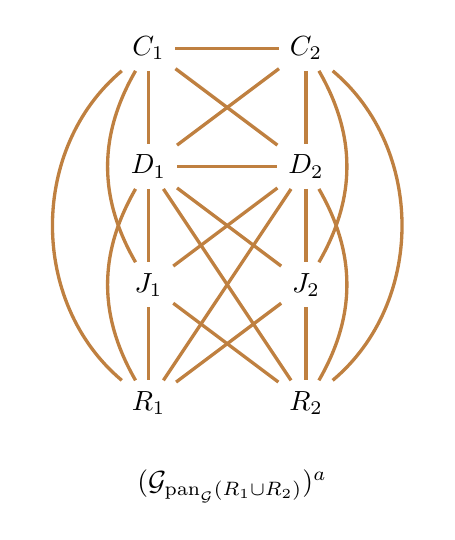
\begin{tikzpicture}[>=stealth, node distance=1.5cm]
		\tikzstyle{format} = [very thick, minimum size=5.0mm, inner sep=0pt]
		\tikzstyle{square} = [draw, very thick, rectangle, minimum size=5.0mm, inner sep=0pt]

		\begin{scope}
		\path[->, very thick]
		node[] (c1) {$C_1$}
		node[below of=c1] (d1) {$D_1$}
		node[below of=d1] (j1) {$J_1$}
		node[below of=j1] (r1) {$R_1$}

		node[right of=c1, xshift=0.5cm] (c2) {$C_2$}
		node[below of=c2] (d2) {$D_2$}
		node[below of=d2] (j2) {$J_2$}
		node[below of=j2] (r2) {$R_2$}
		node[below right of=r1] (label) {$(\G_{\pan_\G(R_1 \cup R_2)})^a$}

		(c1) edge[-, brown] (c2)
		(c1) edge[-, brown] (d1)
		(d1) edge[-, brown] (j1)
		(j1) edge[-, brown] (r1)
		(c1) edge[-, brown, bend right] (j1)
		(c1) edge[-, brown, bend right=50] (r1)
		(d1) edge[-, brown, bend right] (r1)

		(c2) edge[-, brown] (d2)
		(d2) edge[-, brown] (j2)
		(j2) edge[-, brown] (r2)
		(c2) edge[-, brown, bend left] (j2)
		(c2) edge[-, brown, bend left=50] (r2)
		(d2) edge[-, brown, bend left] (r2)
		(d1) edge[-, brown] (d2)
		(c1) edge[-, brown] (d2)
		(c2) edge[-, brown] (d1)

		(d1) edge[-, brown] (j2)
		(d2) edge[-, brown] (j1)
		(d1) edge[-, brown] (r2)
		(d2) edge[-, brown] (r1)
		(j1) edge[-, brown] (r2)
		(j2) edge[-, brown] (r1)
		;
		\end{scope}
		\end{tikzpicture}}
\end{center}
In this augmented graph $(\G_{\pan_\G(R_1 \cup R_2)})^a$, $R_1 \ci_{\text{u-sep}} R_2 \mid \{ C_1, C_2, D_1, D_2, J_1, J_2 \}$.  This implies that $R_1 \ci_{\text{c-sep}} R_2 \mid \pa_\G(R_1, R_2)$ in $\G$ since $ \pa_\G(R_1, R_2)= \{ C_1, C_2, D_1, D_2, J_1, J_2 \}$ . Assuming faithfulness to $\G$ it follows that the term $\odds(R_1, R_2 \mid \text{pa}_\G(R_1, R_2))$ from our factorization above is a valid measure of causal association for this test of the null of no social contagion.
}

{\large\textbf{Problem 4}} (45 points + up to 6 points of extra credit)

This problem contains an analysis component and a programming component. The objective is to help you understand how to move from a novel theoretical result to implementing this idea to gain insights from data.

1) A directed (but not necessarily acyclic) graph $\G$ on $d$ variables $V_1, \dots, V_d$ can be summarized as a $d \times d$ binary adjacency matrix $A$ as follows: $A_{ij} = 1$ if $V_i \diedgeright V_j$ exists in $\G$, and $A_{ij} = 0$ otherwise.\footnote{$A_{ij}$ denotes the $(i, j)$-th entry of the matrix $A$.} Let $e^A$ be defined as the matrix exponential, whose Taylor expansion is quite similar to the standard scalar exponential,
\begin{align*}
e^A = \sum_{k=0}^{\infty} \frac{1}{k!} A^k.
\end{align*}
Prove that $\text{trace}(e^A) - d = 0$ \textbf{if and only if} $\G$ is acyclic, i.e., $\G$ is a DAG, where $\text{trace}(\cdot)$ is the sum of the diagonal elements of the matrix. (7 points)

Hint: you may use the fact that $A_{ij}^k$ counts the number of directed walks of length $k$ from a vertex $V_i$ to $V_j$.

\problemAnswer{
First, note that the following are all equivalent
\begin{align*}
\text{trace}(e^A) - d &= 0 \\
\text{trace}(e^A) &= d \\
\text{trace}(\sum_{k=0}^\infty \frac{1}{k!} A^k) &= d \\
\sum_{k=0}^\infty \sum_{i=1}^d \frac{1}{k!} A_{ii}^k &= d
\end{align*}
First, we show that {\bf if} $A$ is acyclic {\bf then} $\text{trace}(e^A) - d = 0$. Note that if $A$ is acyclic then there exists one and only one path from $V_i \diedgeright V_i$, a path of length zero. Using the hint, we see that
\begin{align*}
\sum_{k=0}^\infty \sum_{i=1}^d \frac{1}{k!} A_{ii}^k &=  \sum_{i=1}^d \frac{1}{0!} A_{ii}^0 \\
&= \sum_{i=1}^d 1 \\
&= d \text{ (QED)}
\end{align*}
Next, we show that {\bf if} $A$ is {\bf not} acyclic {\bf then} $\text{trace}(e^A) - d \neq 0$. Assume $A$ has a cycle of length $l$ from $V_i \diedgeright ... \diedgeright V_i$. Then for $k=l$, there is at least one path of length $k$ from $V_i$ to $V_i$. Noting also that all zero-length paths from $V_i$ to self remain and $\frac{1}{k!}A_{ii}^k \geq 0\ \forall i,k$, we have
\begin{align*}
\sum_{k=0}^\infty \sum_{i=1}^d \frac{1}{k!} A_{ii}^k &= \sum_{i=1}^d \frac{1}{0!} A_{ii}^0 + \sum_{k=1}^\infty \sum_{i=1}^d \frac{1}{k!} A_{ii}^k \\
&= \sum_{i=1}^d \frac{1}{0!} A_{ii}^0 + \sum_{i=1}^d \frac{1}{l!} A_{ii}^l + ... \\
&> \sum_{i=1}^d \frac{1}{0!} A_{ii}^0 = d
\end{align*}
So for any cyclic graph, $\text{trace}(e^A)>d$
}

2) Implement the above constraint as a Python function in the \texttt{hw3.py} skeleton. The function takes as input a binary adjacency matrix in the form of a \texttt{numpy} array. Run the provided test cases to confirm that your implemented constraint is correct. (3 points)

3) For the rest of Problem 4 we will assume that the data are generated from a DAG with a linear Gaussian SEM (Gaussians belong to the curved exponential family) as follows,
\begin{align*}
V_i \gets \beta_0 + \sum_{V_j \in \pa_\G(V_i)} \beta_j V_j + \epsilon_i,
\end{align*}
where noise terms $\epsilon_i$ are drawn from a normal distribution and are mutually independent of each other. That is, each variable is generated as a linear function of an intercept term, its parents, and a Gaussian noise term.

We saw in lecture that the Bayesian information criterion (BIC) is a \textbf{consistent} score for model selection when the underlying data generating process comes from the curved exponential family. Similar to how the joint distribution for a DAG factorizes as a product of conditionals of each variable given its parents -- $p(V_i \mid \pa_\G(V_i))$ -- the BIC score for DAGs also decomposes as the sum of BIC scores for individual models fit for each variable given its parents. That is, for DAGs,
\begin{align*}
\text{BIC} = \sum_{V_i \in V} \text{BIC}_{V_i \mid \pa_\G(V_i)}
\end{align*}
%
Implement the linear Gaussian BIC score for DAGs as a Python function in the \texttt{hw3.py} skeleton as follows. The function accepts an adjacency matrix encoding a DAG, a \texttt{pandas} data frame containing the data, and a Python dictionary mapping row/column indices in the adjacency matrix to variable names in the data frame. For each variable $V_i$, use the structure of the adjacency matrix to fit a linear regression of $V_i$ as a function of an intercept term and its parents using ordinary least squares from the \texttt{ols} module of the \texttt{statsmodels} package. Then, $\text{BIC}_{V_i \mid \pa_\G(V_i)}$ can be directly obtained as an attribute from this fitted model.\footnote{If you're curious about the explicit calculations for the BIC from linear regressions, check out the Gaussian special case of the BIC here: \url{https://en.wikipedia.org/wiki/Bayesian_information_criterion}.} Use the decomposability of the BIC for DAGs as mentioned above to compute the BIC for the entire model. \\(7 points)

4) Run your implemented BIC function on the test cases provided in the \texttt{hw3.py} skeleton and answer the following questions based on the tests. Please provide the computed BICs and answers to the questions \textbf{explicitly} in the PDF submission.

a) Based on their BICs, which of $\G_1, \G_2, \G_3, \G_4$ would you consider to be Markov equivalent? (3 points)

\problemAnswer{
$\G_1, \G_2,$ and $\G_4$ each have a BIC of $23030.573$, while $\G_3$ has a BIC of $22548.647$ \\ \\
This suggests that $\G_1, \G_2,$ and $\G_4$ are Markov equivalent, and $\G_3$ is not Markov equivalent to the rest.
}

b) If the true data generating process is a linear Gaussian SEM corresponding to one of the 4 DAGs, which of the models would the BIC suggest picking as the true underlying model? (3 points)

\problemAnswer{
The BIC decreases as log likelihood increases, and increases as complexity increases, so $\G_3$, which has the lowest BIC, is the best pick for the true underlying model.
}

5)  Similar to HW2, you are provided data that is drawn from the paper by \cite{sachs2005causal} in the file \texttt{data.txt}. Your goal for this homework is to implement a ``causal discovery'' or ``structure learning'' procedure where you will start with an empty DAG (a DAG with no edges) over all of the proteins, and try to find one which fits the data best according to the BIC function you have just implemented. Your implementation of the acyclicity constraint in part 1) will ensure your procedure rejects any graphs that are not acyclic. Ultimately, you will qualitatively compare the DAG learned by your procedure to the one inferred by \cite{sachs2005causal} in the original paper.

A simple procedure to find the DAG with the optimal BIC is to simply enumerate all possible DAGs on the variables provided and pick the ones that have the lowest BIC score. The given dataset contains 10 proteins. The number of possible DAGs on $d$ variables grows super-exponentially -- so, on 10 variables we have 4175098976430598143 possible DAGs! So enumerating all DAGs and scoring them is clearly impossible. Instead, we will implement a greedy approach to causal discovery as follows.


Implement the  greedy causal discovery algorithm in Algorithm~\ref{alg:greedy} (last page of this PDF) using the skeleton provided in \texttt{hw3.py}. (16 points)

\textbf{Helpful tip}: set the number of steps to be low (maybe 10 or so) as you debug your implementation.

\begin{algorithm}[t]
	\caption{\textproc{Causal Discovery}} \label{alg:greedy}
	\begin{algorithmic}[1]
		\vspace{0.5em}
		\State \textbf{Inputs}: ${\cal D}$ pandas data frame, num\_steps (default 100), $\epsilon$ cycle score tolerance  (default $1e^{-9}$)
		\vspace{0.5em}

		\State Initialize empty DAG as $A^*$ a $d\times d$ matrix with all zeros
		\State Initialize an empty set $E$ to store edges in the graph for easy deletion/reversal moves
		\State Set up ${\cal M}$ as a map from row/column indices in $A^*$ to variable names in ${\cal D}$
		\State Initialize $\text{BIC}^*$ as $\text{BIC}(A^*, {\cal D}, {\cal M})$ \Comment{using the function implemented in part 3)}
		\vspace{0.5em}

		\For {$i \text{ in } (1, \dots, \text{num\_steps})$}

		\vspace{0.5em}
		\State There are 3 types of moves we will consider at each step -- random edge \textbf{addition}, random edge

		\hspace{-0.25cm} \textbf{deletion}, and random edge \textbf{reversal}. We will score the BIC of each move and pick the best if it is

		\hspace{-0.25cm} better than the current DAG in $A^*$
		\vspace{0.5em}
		\State For random edge addition:

		\begin{itemize}
			\item Generate random indices $i, j$

			\item Check setting $A^*_{ij}$ to 1 yielding a new matrix $A_{\text{add}}^*$ is still a DAG, i.e., \textproc{Cycle Score}$(A_{\text{add}}^*)< \epsilon$

			\item If it is a DAG, store $\text{BIC}_{\text{add}}$ as $\text{BIC}(A_{\text{add}}^*, {\cal D}, {\cal M})$
		\end{itemize}

		\State For random edge deletion:

		\begin{itemize}
			\item Choose a random edge from the set of existing edges $E$

			\item Set $A^*_{ij}$ to 0 yielding a new matrix $A_{\text{delete}}^*$ (this is guaranteed to be a DAG)

			\item Store $\text{BIC}_{\text{delete}}$ as $\text{BIC}(A_{\text{delete}}^*, {\cal D}, {\cal M})$
		\end{itemize}

		\State For random edge reversal:

		\begin{itemize}
			\item Choose a random edge from the set of existing edges $E$

			\item Set $A^*_{ij}$ to 0 and $A^*_{ji}$ to 1 yielding a new matrix $A_{\text{rev}}^*$ and apply the acyclicity check to $A_{\text{rev}}^*$.

			\item If it is a DAG, store $\text{BIC}_{\text{rev}}$ as $\text{BIC}(A_{\text{rev}}^*, {\cal D}, {\cal M})$
		\end{itemize}

		\vspace{0.5em}
		\State Compare $\text{BIC}_{\text{add}}, \text{BIC}_{\text{delete}}, \text{and } \text{BIC}_{\text{rev}}$ and pick the lowest (best.) Call it $\text{BIC}_{\text{move}}$

		\vspace{0.5em}
		\State If $\text{BIC}_{\text{move}} < \text{BIC}^*$ then apply the move (add, delete, reverse as appropriate) to $A^*$ and the set

		\hspace{-0.25cm} of edges $E$ and update $\text{BIC}^*$ to $\text{BIC}_{\text{move}}$
		\State

		\EndFor
		\vspace{0.5em}
		\State \textbf{return} $A^*, E, {\cal M}$
	\end{algorithmic}
\end{algorithm}

6) Visualize the final DAG learned by running your implementation for $100$ steps. Include an image of the graph in your PDF submission. We have provided you code to do the visualization using the \texttt{Ananke} package in the skeleton \texttt{hw3.py}. If you wish you to use a different package you may do so. Examine the final DAG and write a few sentences about how it compares to the DAG learned by \cite{sachs2005causal} shown in Figure~\ref{fig:prob6}.  E.g., is the $\text{Raf} \diedgeright \text{Mek} \diedgeright \text{Erk}$ cascade present in your DAG? Provide any other comparisons you find interesting. We are not evaluating you on how well your DAG compares to the original one -- it turns out several researchers have tried to recreate it and failed. We just want you to get practice visualizing and interpreting outputs from your code in preparation for the final project. (6 points)

\problemAnswer{
Our DAG appears to be pretty different from that learned by Sachs et al. The Raf $\diedgeright$ Mek $\diedgeright$ Erk cascade is not present in our DAG, we find Mek to be a parent of both Erk and Raf. A notable difference is that our DAG is much more dense than the one Sachs et al. learned, and quite a few of the edges that are shared have reversed orientation (such as aforementioned Raf $\diedgeright$ Mek, as well as Erk $\diedgeright$ Akt). However, one interesting point is that we do also see that PKC and PKA have quite a lot of edges. These types of hubs can be very important in biological networks like this one, so it's worth noting whether some of the same hubs appear, and this would be one potential area for further focus (this association isn't too strong, as Erk for example also has many edges in our graph but not in theirs). This preservation of hubs could be a point to come back to if we were to look at alternative structure learning techniques, especially any that more strictly enforce sparsity.
}

\textbf{Extra credit}: Make the implementation better in any one of the following ways:

\begin{enumerate}
	\item Design a simple new heuristic or move and justify why it might help in addition to the ones already present. Feel free to get really creative here! (3 points)
	\item We know the BIC is decomposable, which means that each edge addition, deletion, or reversal does not require recomputing the BIC for every variable -- only the ones whose parent sets changed. Improve computational efficiency of the algorithm by taking advantage of the BIC's decomposability. Note: you might feel your current procedure is slow, but parallel implementations that take advantage of the decomposability of the BIC have been run on problems with millions of variables! (6 points)
	\item We know the BIC for Markov equivalent graphs are roughly equal. This can be used to keep track of any DAGs we find along the way that are Markov equivalent to our final DAG, as a way of reporting uncertainty in the edge orientations (we will learn more about this in a week or two.) Implement a separate function \textproc{Causal Discovery Equivalence} that augments your causal discovery function to also collect Markov equivalent DAGs in the final solution. We are asking for a separate function here so that it does not mess up our autograder. (5 points)
\end{enumerate}

\problemAnswer{
I implemented number 2 in the function \textproc{Causal Discovery Efficient}. Since the BIC is decomposable into a sum of terms from each node based solely on that node's parents, we can improve efficiency by keeping track of $\text{BIC}^*_{\text{nodewise}}$, a list of $d$ terms, one for each node, such that $\text{BIC}^*_{\text{nodewise}}[i] = \text{BIC}_{V_i \mid \text{pa}_{\G}(V_i)}$. Then for each edge manipulation, we only have to recompute the BIC for the nodes whose parents changed (the tail for edge addition/deletion, both head and tail for reversal) rather than the full graph. This procedure learns the exact same DAG, but runtime improved from 23.1 seconds to 4.165 seconds for 100 steps. This application of the decomposed BIC would scale much better to larger graphs.
}

You can get a max of up to 6 points of extra credit for implementing any one of these (you will not get extra points for implementing multiple bonus features but you can do so if you wish.)



\begin{figure}[h]
	\begin{center}
		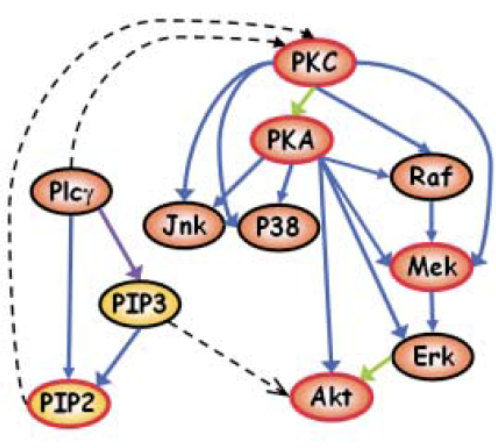
\includegraphics[scale=0.6]{sachs_network}
	\end{center}
	\caption{The DAG learned from phospho-protein/phospho-lipid expression data by \cite{sachs2005causal}}
	\label{fig:prob6}
\end{figure}


\bibliographystyle{apalike}
\bibliography{references}






\end{document}
